%!TEX root = Manuscript.tex

\chapter{Algorithmic and industrial context}
\label{chap:context}
\minitoc

\section{Industrial context}
\subsection{What is 5G ?}



Telecoms networks must manage more and more users while continually improving their bandwidth, latency and reliability. Nowadays, 4G is the standard deployed in most of the territory, and 5G is the new technology under deployment. The term 5G defines a set of functional specifications. The organism that proposes these specifications is the ITU (International Telecommunication Union), an agency of the United Nation responsible for information and communications. For several years, the ITU-R (radiocommunication component of the ITU) has been working to determine the functional aspects that 5G must satisfy. Figure~\ref{fig:5gperf} from~\cite{dahlman20185g} illustrates some of those functional aspects, that ITU-R has formally referenced in IMT-2020 (the requirments of 4G are referenced as IMT-advanced): a bitrate up to 20Gbps ($\times 20$ compared to 4G), low end to end latencies down to 1ms ($10$ times lower than in 4G, we are focusing on this aspect in this thesis).
Also, 5G aims to offer an higher connection density (up to 1 million device$/km^2$), with an higher traffic capacity (from $0,1 Mbit/s/m^2$ in 4G to $10 Mbit/s/m^2$ in 5G) thanks to a wider use of the spectrum. Other aspects as a better energy efficiency ($100$ times better in 5G than in 4G) or a better mobility are required. 

  \begin{figure}[h]
      \begin{center}
      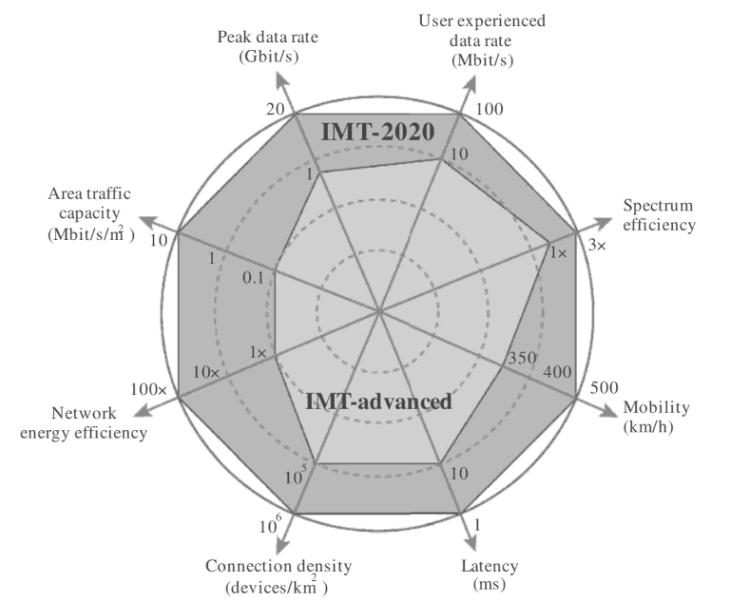
\includegraphics[width=1\textwidth]{Chapitre1/5Grequirements}
      \end{center}
      \caption{5G performances required by ITU-R~(\cite{dahlman20185g})}\label{fig:5gperf}
      \end{figure}

All these characteristics allow various application cases. Figure~\ref{fig:usecases} taken from~\cite{5GACIA} establishes a non-exhaustive list of them, according to their different technical constraints. One of them is \textbf{low latency}, required for applications like motion control that work in real time. Also,  5G aims to develop dynamic programmable networks, for greater flexibility of use. This thesis focuses on developing algorithm to dynamically manage flows in the network in order to provide low latency.

On the other hand, a higher bandwidth is usefull for applications like video streaming, augmented reality or ensuring the connectivity of a large number of terminals. By relaxing latency and bandwidth constraints, it is possible to expand further the number of devices (up to 1 million) for applications like sensors networks.

  \begin{figure}[h] 
      \begin{center}
      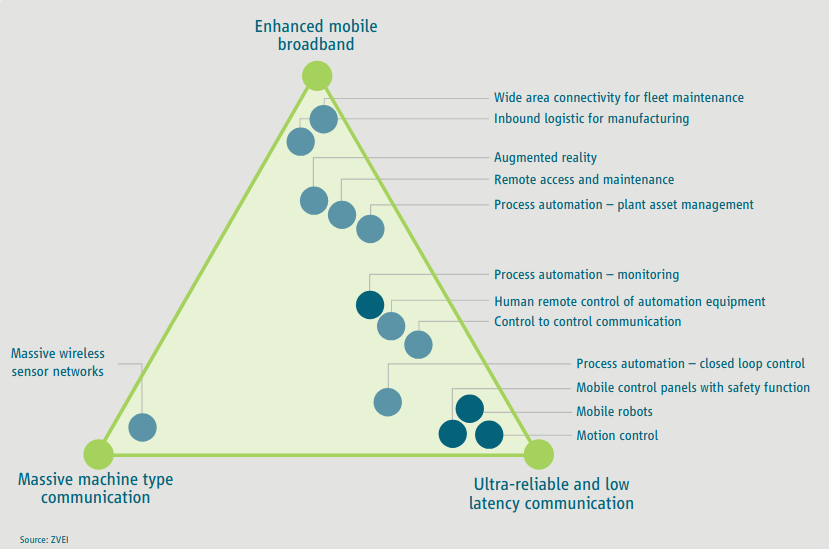
\includegraphics[width=1\textwidth]{Chapitre1/usecases.png}
      \end{center}
      \caption{Some examples of use cases for 5G~(\cite{5GACIA})}\label{fig:usecases}
      \end{figure}



\subsection{Which aspect of 5G do we focus on ?}


To meet these 5G functional specifications, the network equipments must follow technical standards. The 3GPP (3rd Generation Partnership Project) is an union between several standard organizations which defines the technical specifications for 5G. 3GPP regulary publishes releases, that regroup new specifications. The first release focused on 5G was Release 15 (R15), released in 2018~\cite{RELEASENOKIA}.  

  \begin{figure}[h]
      \begin{center}
      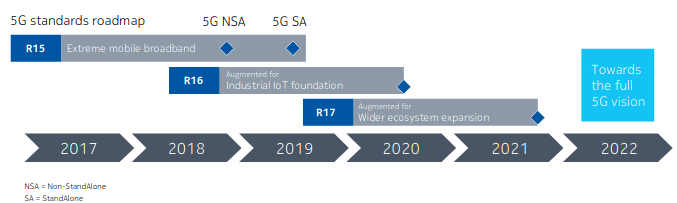
\includegraphics[width=1\textwidth]{Chapitre1/release.png}
      \end{center}
      \caption{3GPP releases 15, 16 and 17 calendar~(\cite{RELEASENOKIA})}\label{fig:release}
      \end{figure}
  

Release 15 focused on increasing throughput and interworking between 4G and 5G, and introduced the notion of URLLC (Ultra-Reliable Low-Latency Communication). URLLC consists in ensuring low packet loss and low latency communications. Indeed, several use cases (smart factories, control operations, \dots) needs highly reliable communications in which the latency must be guaranteed. 
The objective of this thesis is to compute schemes for low latency communications. To do so, the network equipments must be able to manage the traffic by discriminating different kinds of flows and following the computed schemes to manage them. Even if current network does not yet have such capabilities, releases 16 an 17 have deepened the notion of URLLC and this topic is widely studied. 

\subsection{Current way to manage networks : Statistical Multiplexing}


The constraints expressed for low latency architectures and 5G standard are hard to meet in current networks. In IP or even Ethernet networks, the traffic usually suffers of delay due to contention. 

As we just mentioned, the current network nodes (routers for IP networks, switches for Ethernet networks) are not able to schedule packets. The only function of the nodes is to forward the packets to the right output port.
The objective is to offer a good average quality of service for a minimal price. When a single input flow uses an ouput port, there is no issue.
 If several packets comming from several flows require the same output port at the same time, we talk about \textbf{contention}. Some packets are then put in a \textbf{contention buffer} until the port is available. The additional latency induced by contention buffers is one of the most important causes of delay. In order to avoid this situation, the bitrates of the links is dimensioned according to the use case. It is then calculated according to the average bitrate of the flows on the network. 
 When there is too much packets in the buffer, the oldest packets of the buffer are \textbf{lost}. 

Such a technology ensures an easy deployment and managment of the networks and most of the time a good quality of service for a minimal cost for network providers, but it may induce packet losses and high latencies. Hence, we talk about statistical multiplexing~\cite{krishnamurthy2003latency,venkatramani1994supporting}. \todo{pourquoi hence, plutot dire ce qu'on vient de décrire est appelé statistical multplexing}

URLLC aims to ensure good end to end latency communications. To achieve such a goal, each component of the communication network must satisfy a low latency: the radio communications, and the core network. This thesis focus on the core network. 

\subsection{\textbf{R}adio \textbf{A}ccess \textbf{N}etwork}

To understand the network this thesis focuses on, we now describe how a radio access network works.

Current mobile network (aka cellular network) architecture consists in a distributed radio access networks: the mobile terminals connect to a base station (BTS for Base Transceiver Station as a generic name, eNB for evolved Node B in 3GPP LTE “4G” standard or gNB for 5G) that encompasses all the sub-systems needed to realize mobile communication~\cite{bouguen2012lte}. It mainly comprises the radio part, that furnishes the connection between the mobile terminal and the BTS, and the network part that provides control and management functions like mobility support (the main functionality being the support of handover from one BTS to another, i.e. the ability to pursue a communication when moving from the range of an antenna to another).
The BTS are connected together by the Aggregation Network of the operator, itslef connected to the core network, in order to ensure communications with other operators RANs. Figure~\ref{fig:RAN} illustrates a communication between two mobiles using a different operator.

\begin{figure}
\begin{center}
\scalebox{0.4}{

\begin{tikzpicture}
  \SetGraphUnit{5}
    \tikzset{
  EdgeStyle/.append style = {->} }
   \tikzstyle{VertexStyle}=[shape = circle, draw, minimum size = 30pt]
 

  \node (p1) at (0,4) {
\includegraphics[width = 1cm]{phone.png}};
 
  \node (p2) at (0,2) {
\includegraphics[width = 1cm]{phone.png}};

  \node (p3) at (0,0) {
\includegraphics[width = 1cm]{phone.png}};
  
 \node (a1) at (7,1) {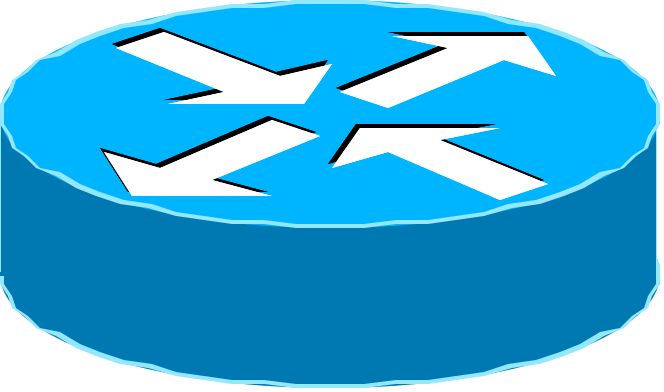
\includegraphics[width = 1cm]{switch.png}};
 \node (a2) at (7,3) {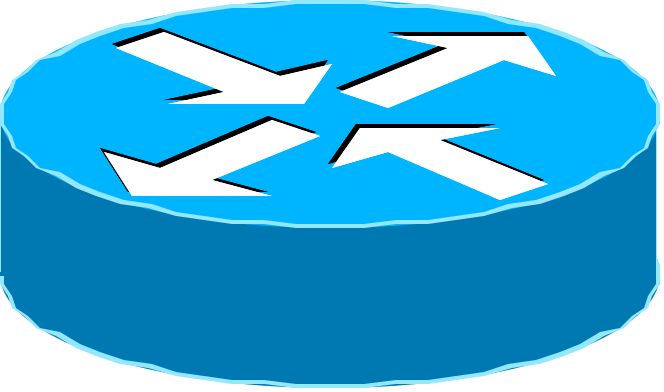
\includegraphics[width = 1cm]{switch.png}};
 \node (a3) at (9,1) {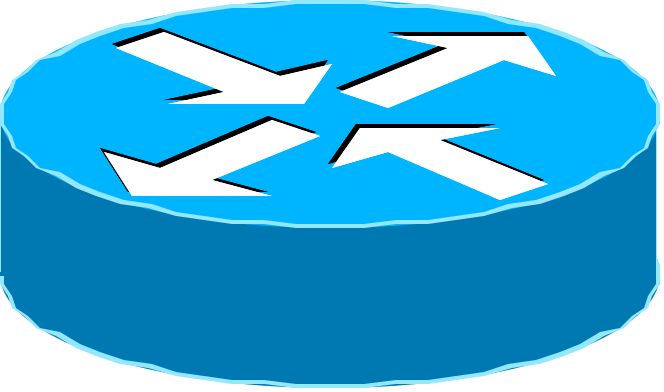
\includegraphics[width = 1cm]{switch.png}};
 \node (a4) at (9,3) {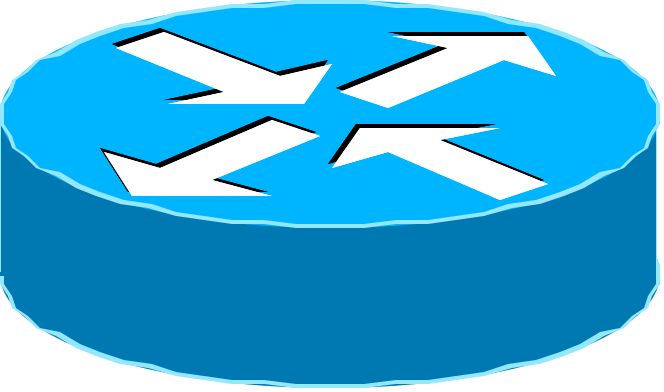
\includegraphics[width = 1cm]{switch.png}};

 \node (c1) at (12,3) {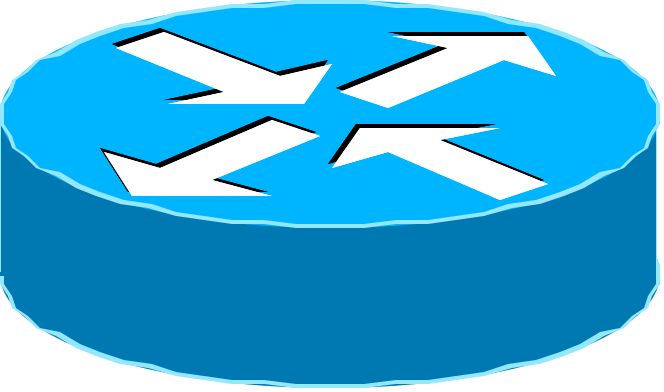
\includegraphics[width = 1cm]{switch.png}};
 \node (c2) at (12,5) {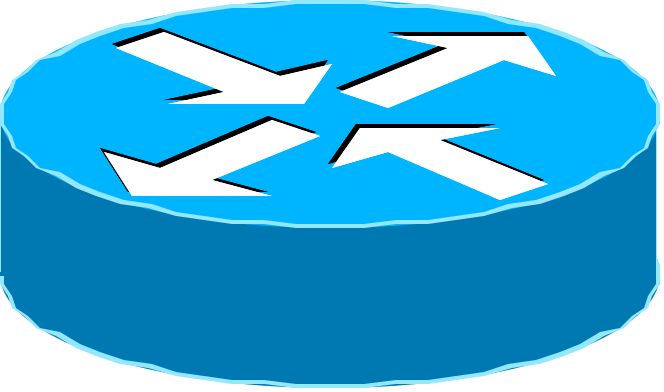
\includegraphics[width = 1cm]{switch.png}};
 \node (c3) at (14,3) {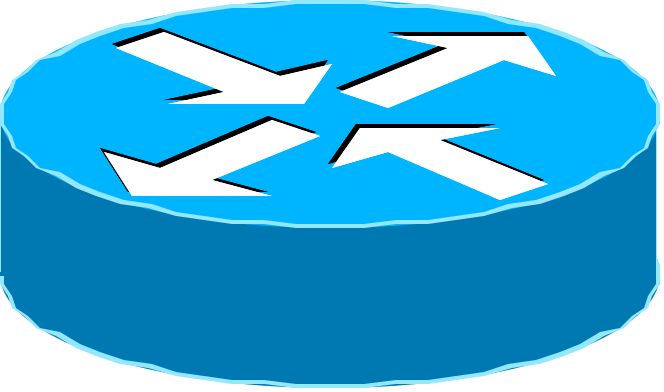
\includegraphics[width = 1cm]{switch.png}};
 \node (c4) at (14,5) {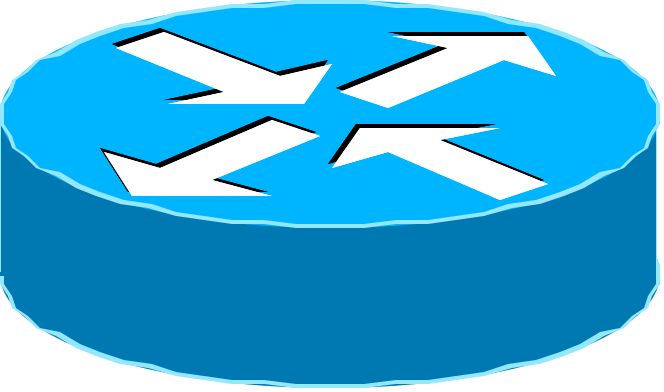
\includegraphics[width = 1cm]{switch.png}};

 \node (a5) at (17,1) {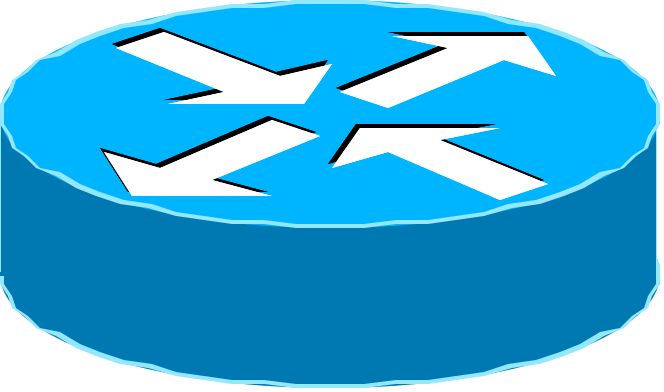
\includegraphics[width = 1cm]{switch.png}};
 \node (a6) at (17,3) {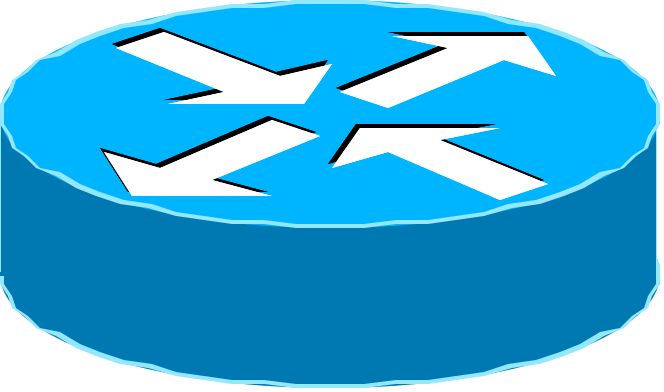
\includegraphics[width = 1cm]{switch.png}};
 \node (a7) at (19,1) {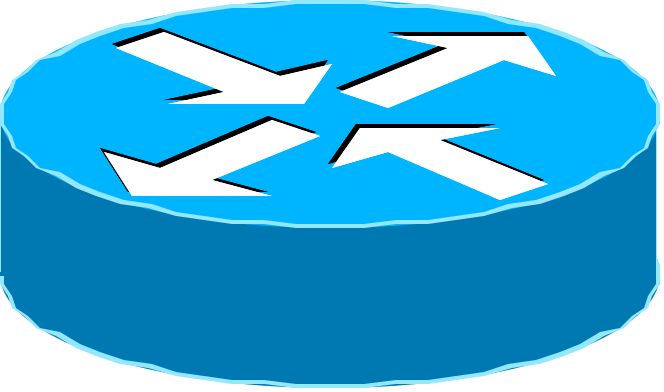
\includegraphics[width = 1cm]{switch.png}};
 \node (a8) at (19,3) {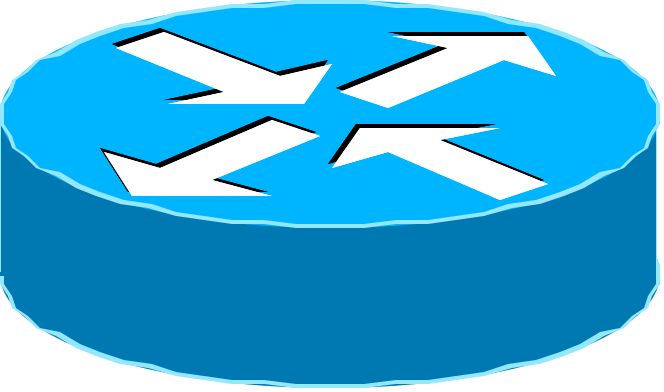
\includegraphics[width = 1cm]{switch.png}};


 \node (p4) at (26,4) {
\includegraphics[width = 1cm]{phone.png}};
 
  \node (p5) at (26,2) {
\includegraphics[width = 1cm]{phone.png}};

  \node (p6) at (26,0) {
\includegraphics[width = 1cm]{phone.png}};
  
   \node (r1) at (4,2) {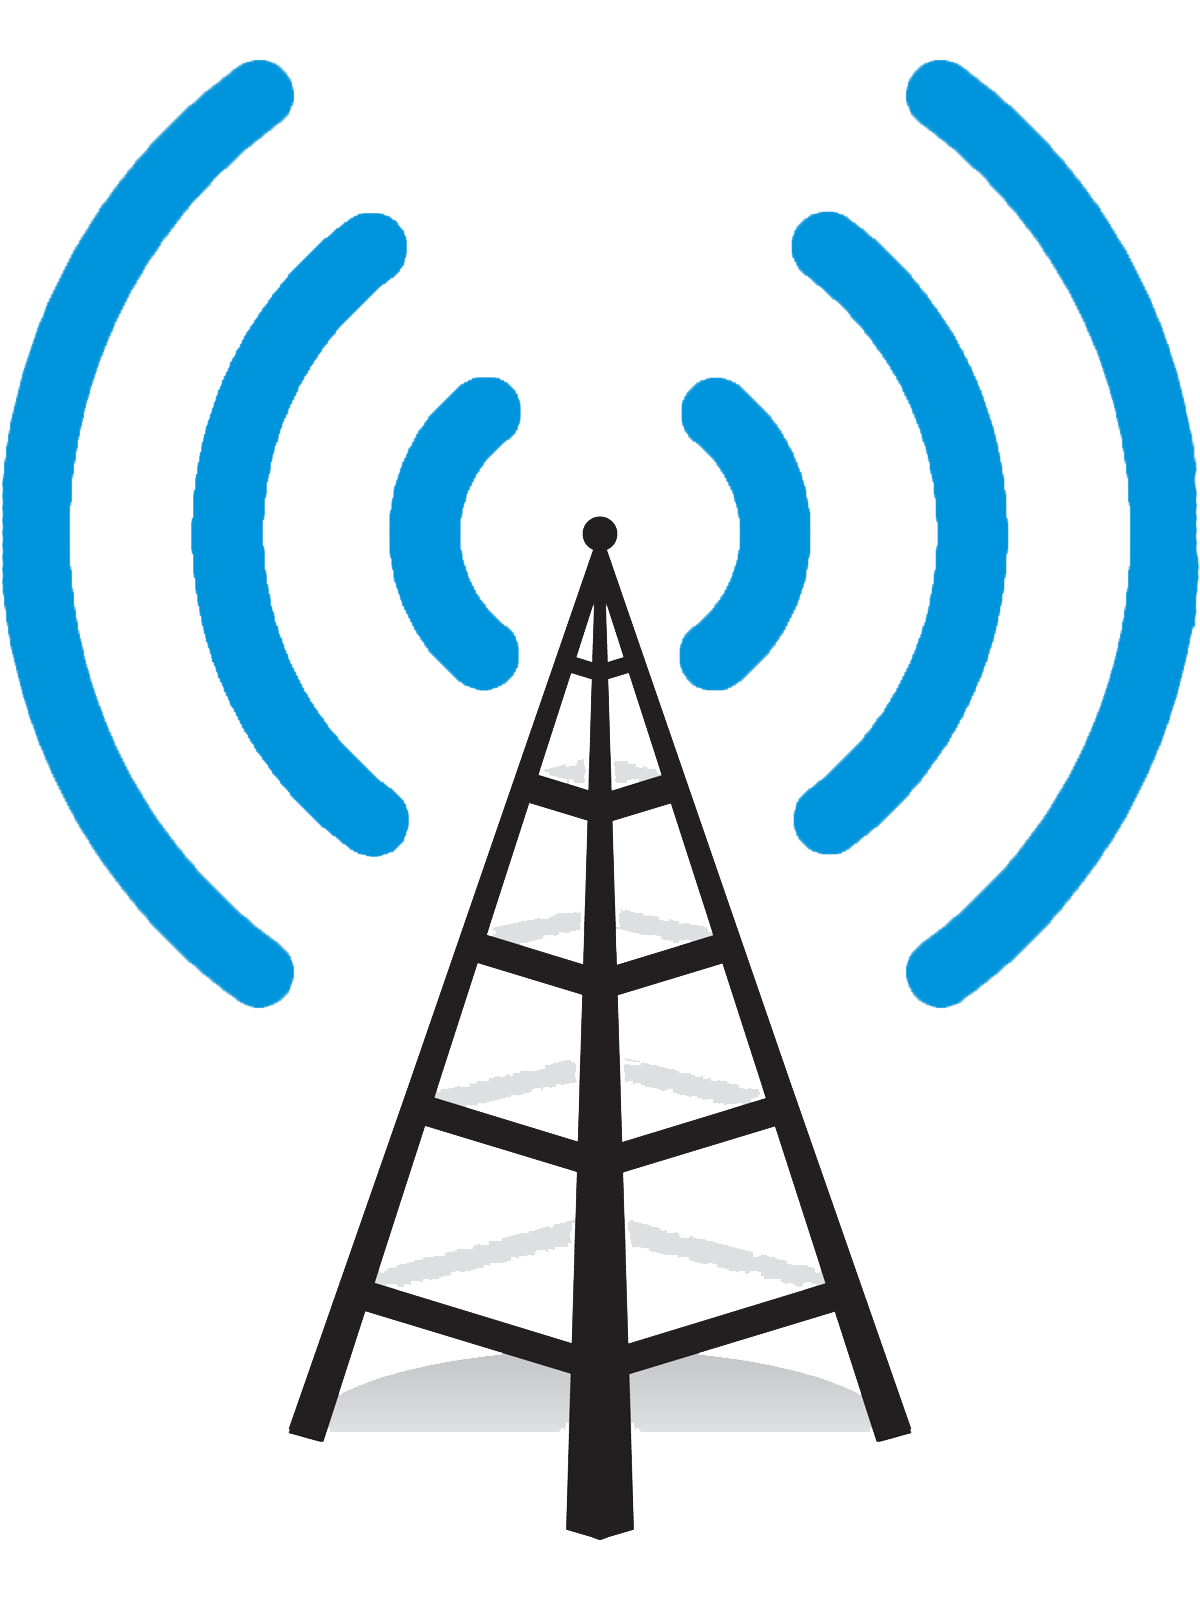
\includegraphics[width = 1cm]{rrh.png}};
   \node (r2) at (22,2) {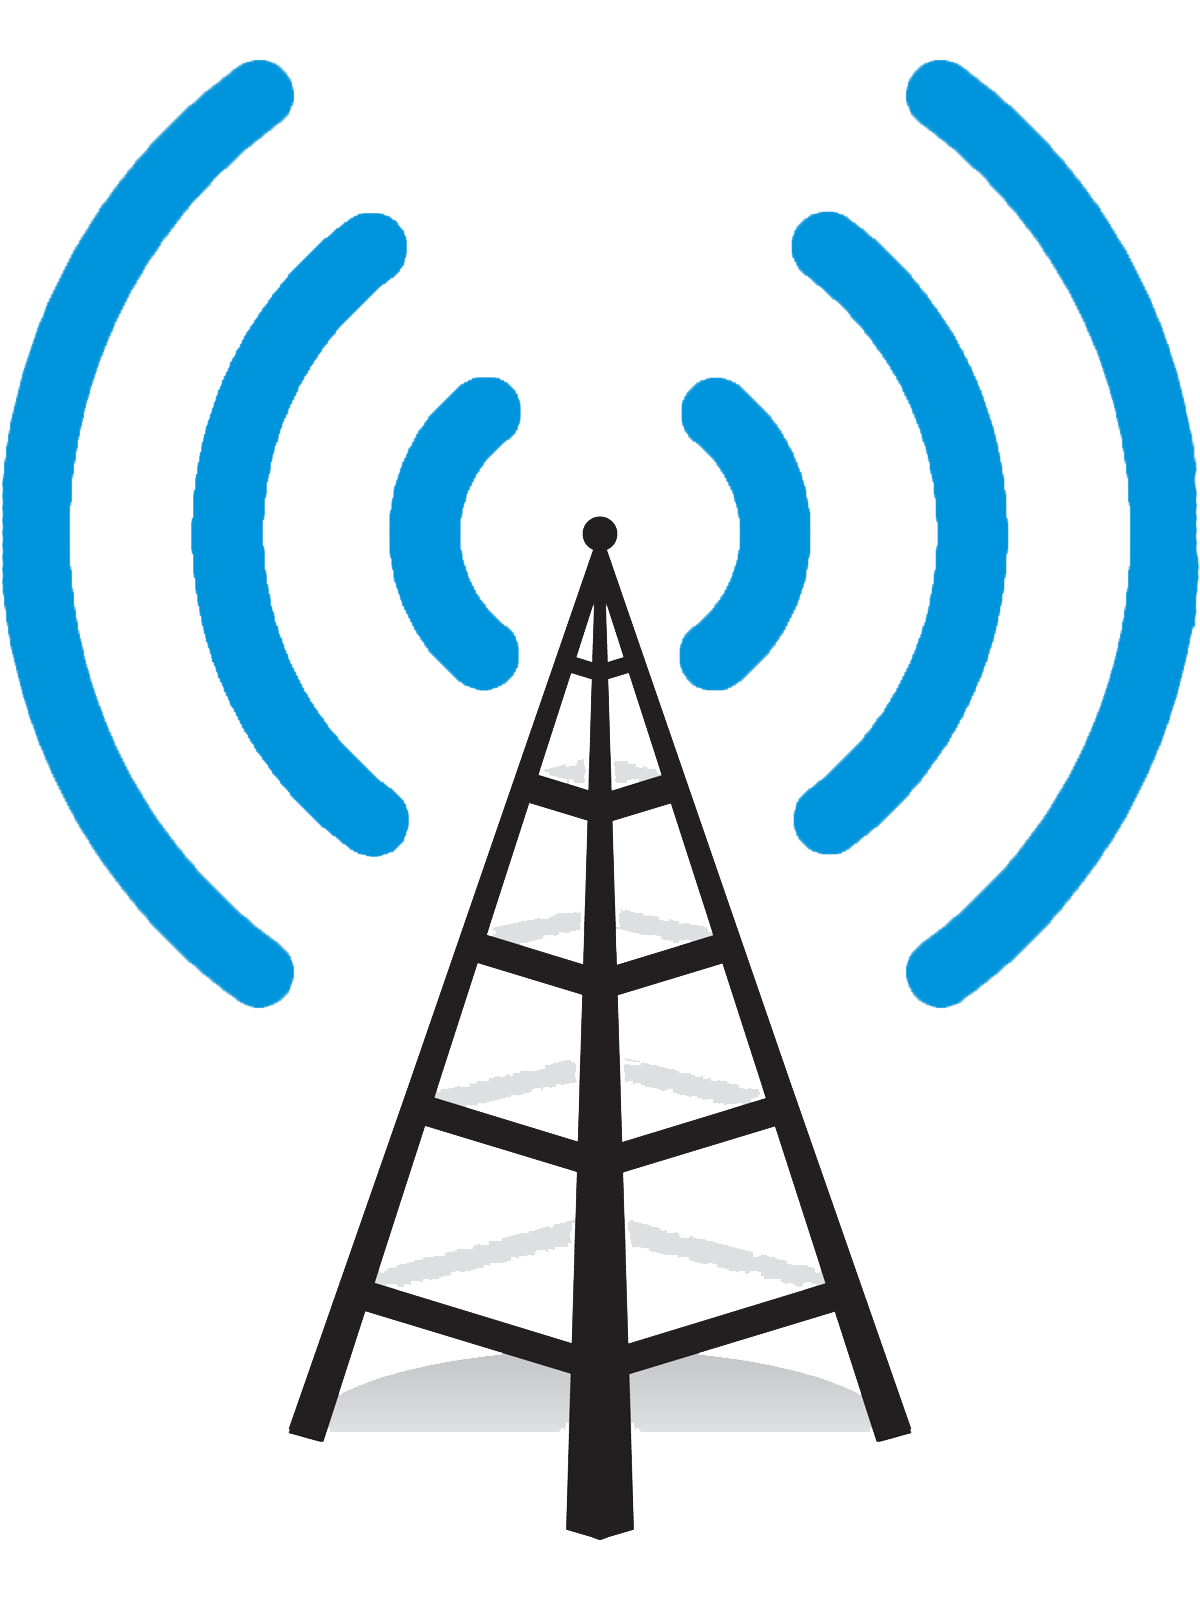
\includegraphics[width = 1cm]{rrh.png}};
   

 
\path (p1) edge [<->,color=red]  (r1);
\path (p2) edge [<->]  (r1);
\path (p3) edge [<->]  (r1);

\path (r1) edge [<->,color=red]  (a1);
\path (r1) edge [<->]  (a2);

\path (a1) edge [<->]  (a2);
\path (a3) edge [<->]  (a2);
\path (a4) edge [<->]  (a2);
\path (a3) edge [<->]  (a4);
\path (a3) edge [<->]  (a1);
\path (a4) edge [<->,color=red]  (a1);


\path (c1) edge [<->]  (c2);
\path (c3) edge [<->]  (c2);
\path (c4) edge [<->]  (c2);
\path (c3) edge [<->]  (c4);
\path (c3) edge [<->]  (c1);
\path (c4) edge [<->,color=red]  (c1);


\path (a5) edge [<->]  (a6);
\path (a7) edge [<->]  (a6);
\path (a8) edge [<->,color=red]  (a6);
\path (a7) edge [<->]  (a8);
\path (a7) edge [<->]  (a5);
\path (a8) edge [<->]  (a5);

 
\path (p4) edge [<->]  (r2);
\path (p5) edge [<->,color=red]  (r2);
\path (p6) edge [<->]  (r2);


\path (a4) edge [<->]  (c2);
\path (a3) edge [<->]  (c1);
\path (a3) edge [<->]  (c2);
\path (a4) edge [<->,color=red]  (c1);


\path (a6) edge [<->,color=red]  (c4);
\path (a5) edge [<->]  (c3);
\path (a5) edge [<->]  (c4);
\path (a6) edge [<->]  (c3);

\path (r2) edge [<->,color=red]  (a8);
\path (r2) edge [<->]  (a7);
\draw[dashed] (-1,-1) rectangle  (10,7);
\node at (5.5, 6.5) {\huge Operator $1$};
\node at (3, 4) {RAN};
\node at (8, 4) {Aggregation};

\draw[dashed] (16,-1) rectangle  (27,7);
\node at (22.5, 6.5) {\huge Operator $2$};
\node at (23, 4) {RAN};
\node at (18, 4) {Aggregation};

\draw[dashed] (11,2) rectangle  (15,7);
\node at (13, 6.5) {\huge Core};

\end{tikzpicture}
}




 \caption{An End to End communication between two mobiles.}

\label{fig:RAN}
\end{center}
\end{figure}


\subsubsection{Cloud RAN}

One possible direction for next generation networks is to become centralized radio network architectures (C-RAN, for Cloud Radio Access Network) to reduce consumption costs and power at the base stations~\cite{mobile2011c}. These C-RAN architectures include simplified base stations on the field. Depending on the architecture choice, it can be restricted to the radio part and the digital to analog conversion only. This can be identified by different names depending on the reference document, including \textbf{RU} for Remote Unit or \textbf{RRH} for Remote Radio Heads. The latter will be used in the thesis. The other components of the C-RAN  are the processing units. One can distinguish two levels of processing units: the \textbf{DUs}, for Distributed Units that are able to ensure only a part of the computation tasks, and the \textbf{CUs} for Centralized Units that computes the most centralized tasks. In this thesis, we consider only CUs, that are also called \textbf{BBUs} for BaseBand Units, and we use this term in the thesis. The BBUs are located in the cloud. 

 \begin{figure}[h]
      \begin{center}
      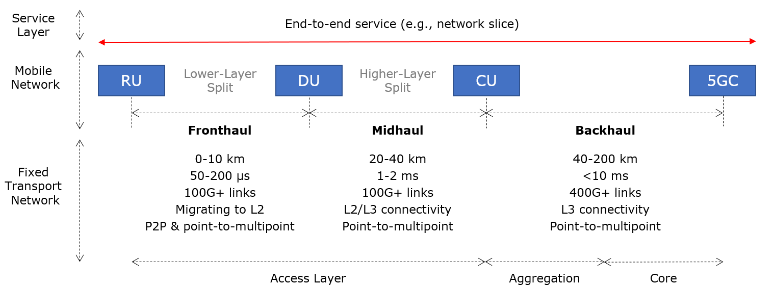
\includegraphics[width=1\textwidth]{Chapitre1/5gran.png}
      \end{center}
      \caption{Latency requirments between different part of the network.}\label{fig:5gran}
      \end{figure}

By cloud we mean the capability of instantiating executable programs in data centers that are transparently connected to the systems requiring the results of the program execution.
 The execution may be indifferently performed on virtualized machines, or bare metal, or any combination of the two. The network between RRHs and BBUs is called “Fronthaul Network”, or “Fronthaul” for short. Figure~\ref{fig:fronthaul} illustrates an example of fronthaul in which several BBUs are gathered in the same datacenter. 

  \begin{figure}[h]
      \begin{center}
      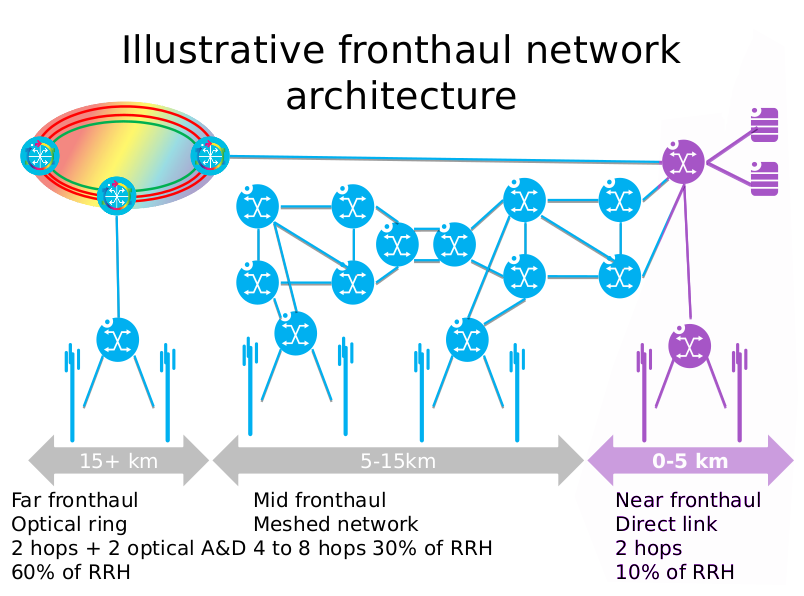
\includegraphics[width=1\textwidth]{Chapitre1/fronthaul.png}
      \end{center}
      \caption{An example of fronthaul network for Clound RAN}\label{fig:fronthaul}
      \end{figure}
      
      \subsubsection{Split}

      As mentioned above, in C-RAN, most of the computation tasks of the BTS must be centralized in the BBU. There are several components that can be centralized, but the more we centralize the ressources, the higher the latency constraints are.
      Figure~\ref{fig:CRANsplit} illustrates two different choices of split for the BTS. The first one, called ``Full centralization'' leaves only the radio functions to the RRH, while the second one, called ``partial centralization'', keeps the baseband processing function inside the RRH. The methods presented in this thesis allow to send an high amount of data in the network while minimizing latency. Such a result matches well with the first split, this is why we talk about BaseBand Units (BBU) here. Even if we choose to work with the most critical split, the amount of data is just a parameter of the problem presented here, and any kind of split could be managed by our algorithms.
      
   \begin{figure}[h]
      \begin{center}
      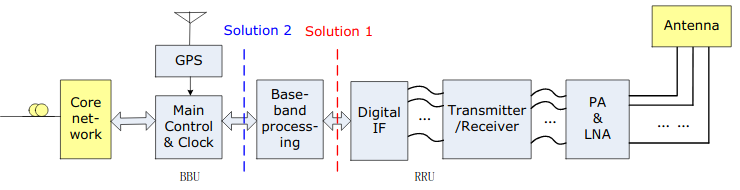
\includegraphics[width=1\textwidth]{Chapitre1/CRANsplit.png}
      \end{center}
      \caption{Two different split for Cloud-RAN}\label{fig:CRANsplit}
      \end{figure}
      \begin{figure}[h]
      \begin{center}
      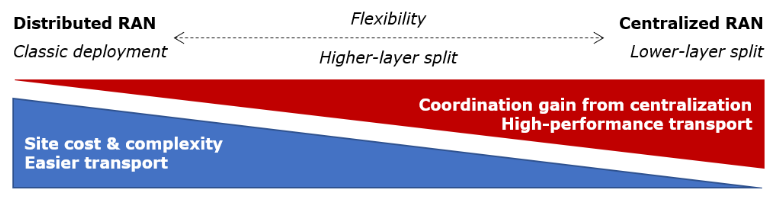
\includegraphics[width=1\textwidth]{Chapitre1/flexibility.png}
      \end{center}
      \caption{The more centralized is the RAN, the hardest is the transport and the lowest is the cost of coordination for the antennas}\label{fig:flexibility}
      \end{figure}
       
This kind of architecture must address the problem of the latency in the transfer process between the RRHs on the field and BBUs in the cloud. Low latency is already critical for the deployment of C-RAN approach in LTE “4G” networks. The standard requires hard time constraints for functions like HARQ (Hybrid Automatic Repeat reQuest) that needs to be processed in less than $3ms$ \cite{bouguen2012lte}. Considering processing time into the BBU, the time budget over the network can be as low as $400\mu s$ for a round trip. One specificity in this C-RAN context is not only the latency constraint, but also the periodicity of the data transfer between RRH and BBU (this HARQ constraint must be enforced for each frame emitted every millisecond). Looking beyond current mobile network generation, one must have in mind that upcoming 5G standards will require to reach end-to-end expected latency as low as $1ms$ (depending on targeted services)~\cite{boccardi2014five}. New schedulings and new technologies have to be considered to guarantee delay constrained periodic data transfers. 


\subsection{Technical solution for low latency}

Statistical multiplexing is the most common mechanism used to manage packet based networks in the last $40$ years. While IETF tools~\cite{metricsietf} ensure a latency lower than a given value for $95\%$ of the packets, such a guarantee is not sufficient in our context in which all packets must satisfy latency constraints. While there are mechanisms which can be used to prioritize some packets over the others (e.g. Express Forwarding~\cite{exprforw} against Best Effort), they fail to guarantee the delivery of a given packet in a given time delay when several packets compete for the same resource. 


The best current solution is to rely on an almost full optical approach, where each end-point (RRH on one side, BBU on the other side) is connected through direct fiber or full optical switches~\cite{pizzinat2015things,tayq2017real}. This architecture is very expensive and hardly scales in the case of a mobile network. As illustrative purpose, a single (one operator) mobile network in France is composed of about $10,000$ base stations. This number will increase by a factor of $2$ to $20$ with the emergence of “small cells” which increases base station density to reach higher throughput \cite{leclerc2016transmission,leclerc2016signaling}. It is thus needed to find a solution to offer low latency over commoditized packet based networks. 

Although 3GPP standards for 5G are not completely frozen yet, the core network is designed to use ethernet technology. Time Sensitive Networking (TSN)~\cite{ieee802,ieeep802} is a task group of IEEE that develops some standards for ethernet. We focus on several of those standards which allow a control of the latency.
 The model and the algorithms of this thesis make the hypothesis that the network components are syncrhonized, able to collect some information and send it to a centralized entity, to differentiate several kinds of flow and to forward it at an exact date, imposed by the controller. TSN standards propose technical solution for those hypothesis, but an approach like TSN is still based on statistical laws and is limited to ensure a perfect control of the latency. Indeed, TSN allows a bounded latency but not a minimal latency. The limits of TSN and the technical solution we propose are detailled in Chapter~\ref{chap:TSN}.

 In this thesis, we work on deterministic flows. Thus, we propose algorithms to compute deterministic scheduling on the flows in the network, while minimizing the latency due to buffering. Remark that minimizing the buffering latency allows not only to meet latency constraints of applications, but also to leave additional time for others sources of latency (additional computations, longer length of fibers, etc...)



\section{Algorithmic related works}
 
 We first shortly describe the algorithmic problems described in Chapter~\ref{chap:model} studied in this thesis. We consider a network in which the routing is fixed. Several flows share the network, sending periodically a message of the same size from a source to a target. This message represents several packets in practice, but in our model we consider them contiguous. The messages can also be buffered in the nodes of the network in order to let another more critical message use a shared ressource. The objective is to compute the buffering time of every message in the network, such that the global latency (i.e. the largest latency of a flow) is minimal. Note that the periodic aspect of C-RAN makes the problem more difficult. Indeed, since the traffic is periodic and the network highly loaded, we must deal with contentions coming from successive periods while computing the scheduling. There are several variation of the problem according to the shape of the network, the synchronization of the messages in a period or constraints on buffering.
 
 We present in this section several families of problems and approach, which are close to what is presented in this thseis but which
 usually fail to model our problem faithfully or which are too general to derive useful algorithms.


\subsection{Algorithmic Approaches}

\paragraph{Wormhole}
Because we consider contiguous messages, we first focused on wormhole problems~\cite{ni1993survey,cole1996benefit}. Wormhole problems consider graphs representing interconection networks, in which the vertices are the nodes of the network and the edeges are the physical links. Long messages are sent in the network, accaparing ressources during a long time. A \emph{deadlock} occurs when several messages are waiting each others to release a ressource. The main problem consists in avoiding deadlocks. The algorithmic solution proposed consists in multiplexing the physical channels in several virtual channels, and to develop routing algorithms to determine the virtual channel used by each message. In our model, we consider the routing given. Also, our messages require the entire capacity of the links. Furthermore, this problem differs from ours since deadlocks can not occurs in the networks we model in which the routing are considered \textbf{coherent}\cite{Schwiebert1996ANA}. A routing is considered as coherent if two routes share only one path (i.e. a sequence of contiguous links) in the network.

On a technical aspect, whormole switches~\cite{cole1996benefit} are designed to read only the header of the messages before forwarding it instead of buffering the entire messages as in store-and-forward~\cite{tindell1992store}. This method have a huge impact on the latency, particulary on long messages, and we go further by removing every buffering in the switchs.


\paragraph{Graph coloring for ressources allocation}
One of our approach consisted in representing the shared ressources of the network by a conflict graph. The vertices of the graph represent the routes of the networks and there is an edge between two vertices if their associated routes share the same ressource (i.e. an output port on a switch). The edges of the graph are labeled by the difference of the physical length of the links between the sources of the routes and the conflict point. A proper coloring of such a graph is a scheduling of the network without collisions between the messages. Several graph colorings have been introduced to model similar problems. In~\cite{erlebach2001complexity} the objective is to minimize the number of wavelength in shared links for optical networks. Paper~\cite{borndorfer1998frequency}, introduces flows allocations problems for ressource allocation of the frequencies in radio networks. Unfortunately, they do not take into account the periodicity of the scheduling and the associated problems are already $\NP$-complete. 

\paragraph{Circular Coloring}
The only coloring taking into account periodicity is the circular coloring~\cite{ZHU2001371,zhou2013multiple}. As an example, circular coloring for a road intersection proposes a graph in which the vertex are the flows and there is and edge between two vertices if the flow must not overlap. Such an approach is close to our problem on a single point of the network. However, since the problem is $\NP$-hard and the model is too far from our general graphs, this approach did not catch our attention.
Circular arc coloring~\cite{10.2307/2100446} also manages messages that can be related to periodic messages. The authors consider a clock and several arcs around this clock, representing the time needed by a job. The objective is to find the minimal number of men needed to complete the job. If two arcs overlap, the same man cannot be affected to both jobs. Nevertheless, this problem has been shown $\NP$-hard~\cite{10.1007/BFb0053971} and the model is really far from ours.

\subsection{Scheduling approaches}


\paragraph{Train Scheduling}

The train timetabling problem~\cite{lusby2011railway} and its restriction, the periodic event scheduling problem~\cite{serafini1989mathematical} are generalizations of the problem we study. Indeed, they take the period as input and can express the fact that two trains (like two messages) should not cross. However, they are much more general: the trains can vary in size, speed, the network can be more complex than a single track and there are precedence constraints. Hence, the numerous variants of train scheduling problems are very hard to solve (and always $\NP$-hard). Most of the research done~\cite{lusby2011railway} is devising practical algorithms using branch and bound, mixed integer programming, genetic algorithms\dots

\paragraph{Linear Programming for Latency Constrained Network}
We define in this thesis a simple network topology called the {\em star shaped network}. In star shaped networks, all flows goe through the same link, and there is only two relevant contention points (one in the way to the BBUs, and one in the way back to the RRHs).

Variation on the problem of scheduling periodic messages for Cloud-RAN have been investigated in~\cite{nayak2017incremental,steiner2018traffic,silviu2017,naresh2016}. In those papers authors study the practical problem of scheduling a few number of flows on star shaped networks. Given a network in which the routing is set, the objective is to schedule several flows whith a critical latency and several best-effort flows in the same networks. To do so, the authors use new technical standards (detailled in Chapter~\ref{chap:TSN}) that allow to prioritize flows, and linear programming in order to compute a schedule between the critical flows. In the same spirit, an SMT solver is proposed in~\cite{dos2019tsnsched}. Such an approach is still based on statistical models and just ensure that the packets have an end-to-end latency lower than a given value. In this thesis, we focus on minimizing the latency of critical flows, even when there is some best effort traffic as show in Chapter~\ref{chap:BE}. Furthermore, linear porgramming does not scale neither with the number of route nor the number of conflict point on each routes while we propose polynomial algorithms that give satisfying solution on every kind of topology.



\paragraph{Processors Scheduling}

%d'abord le single processor scheduling
%puis le two flow shop problem
%enfin si tu veux les multiples processors, mais je crois que tu dis des bêtises dessus


The problem we address in this thesis is similar to classical single pocessor scheduling problems, defined as follows. Given a set of jobs, a release time and a deadline for each job, find a scheduling to minimize the global completion time (i.e. the time at which all job have been processed). On the star routed network studied in Chapter~\ref{chap:PAZL}, the problem is similar to a two flow-shop scheduling problem. In two flow-shop scheduling, the objective is to schedule the jobs on two processors, each job must be first processed by the first processor and can then 
be processed by the second one after a delay which depends on the job. This two-flow shop problem is $\NP$-hard~\cite{yu2004minimizing}, and while it can be reduced to the synchronized version of our problem, presented in~\ref{chap:SPALL}, the correspondence is less clear with the unsynchronized version of Chapter~\ref{chap:PAZL}. Moreover, our problem adds the constraint of periodicity which makes the model unsuitable.

Scheduling on multiple processors does not seem related to our problems. In~\cite{korst1991periodic,hanen1993cyclic,aupy2017periodic}, several processors are available in parallel and the aim is to minimize the number of processors on which the periodic tasks are scheduled. To our knowledge, there is no problem of periodic scheduling on a networks of processors which can model our network. 


 A survey about cyclic scheduling~\cite{levner2010complexity} explains that in cyclic scheduling problems, the aim is to minimize the period of a scheduling to maximize the throughput, while our period is fixed. 


\paragraph{A polynomial algorithm for single processor scheduling}

The approach we adopt in Chapter~\ref{chap:PALL} to solve our problem on a star routed network, is a two stage approach. The second stage,
when forgetting about periodicity, is similar to a scheduling problem with a single processor with the goal of minimizing the completion time (makespan). The algorithm described in~\cite{simons1978fast}, solves this problem in polynomial time when all tasks have the same processing time. We use it as a building block of several of our algorithms in Chapter~\ref{chap:PALL} and
Chapter~\ref{chap:SPALL}, where we adapt it to the case of periodic jobs. When the jobs have different processing times, the problem
is $\NP$-hard~\cite{lenstra1977complexity}.


%Attention, tu parles déjà de la thèse
% Algorithm \MLS runs in $O(n^2\log(n))$ and the solution it gives are optimal, that means each job respects its release time and deadline and \emph{the makespan}, that is the time before completion ofthe whole process, is minimimal. Nevertheless, there is still the periodicity constraint to take into consideration. To deal with the periodicity, we propose a greedy algorithm that adapt the deadlines and calls \MLS $n$ times ($n$ is the number of routes in the network). This greedy algorithm does not ensure an optimal solution, and may fail on some instances. We then propose an FPT algorithm which calls \MLS $2^n$ times and gives the optimal solution for our problem on star shaped networks.


\subsection{Conclusion}
One of the trend of 5G and networks in general is to be able to ensure end to end communication with a low latency. To do so, it is important to precisely control the traffic in each part of the network. In this thesis, we focus on the ethernet network. Several technical solutions are currently in development to control the trafic more precisely than statistical multiplexing. The switches requires a precise scheduling of each flow of the traffic and adapt the output traffic following this scheduling. 
In this thesis, we study the problem of computing the scheduling. Knowing the topology of the network, and the different flows it supports, our objective is to compute the periodic scheduling of the traffic for every node of the network, while minimizing the latency of the longest flow. 
%The periodicity of the flows increases the difficulty of the problem.



